\subsection{Mikrocontroller}
\subsubsection{Allgemein}
Der Mikrocontroller ist die Basiskomponente des Edubot Modells. Er nimmt eingehende Verbindungen aus dem Netzwerk an, ermöglicht den Empfang von Positionsdaten, die entsprechende Umwandlung und Ausgabe in Form eines Taktsignals an den digitalen Ausgängen, sowie die Rückmeldung des aktuellen Status an den Computer.

Die Verwendung eines Mikrocontrollers wurde notwendig, da unter Microsoft Windows sehr viele Prozesse gleichzeitig ausgeführt werden und der Thread zur Taktausgabe daher in unregelmäßigen Abständen ausgeführt wird. Damit wird auch die Ausgabe des Taktsignals instabil.

Der von uns verwendete Mikrocontroller wurde von der Firma GHI vertrieben, trägt als genaue Bezeichnung GHI Embedded Masters Breakout Bord v1.0 und verfügt über einen Prozessor in ARM Architektur, sowie diverse Ein- und Ausgänge. Im Funktionsumfang des gewählten Mikrocontrollers ergäben sich auch verschiedene Möglichkeiten wie der direkte Anschluss eines LCD Pannels oder auch externer persistenter Speichermedien wie USB Sticks. Aus diesem Grund finden sich unter den Pins des Controllers zahlreiche speziell für diese Anwendungszwecke bestimmte Ausgänge, welche jedoch bei diesem Projekt nicht verwendet wurden.

Zum Überspielen der Software, die Vornahme von Updates oder zur Durchführung der Fehlerbehebung verfügt der Mikrocontroller über einen USB Anschluss. Des weiteren verfügt der Controller über einen Netzwerkanschluss mit RJ-45 Stecker über den Socket Verbindungen aufgebaut und Daten übertragen werden können.

Grundsätzlich ist die Programmierung des Mikrocontrollers mithilfe des .Net Micro Frameworks von Microsoft über die Entwicklungsumgebung Visual Studio vornehmbar. Der über das .Net Micro Framework ausgeführte Programmcode stellt jedoch keine optimale Performance zur Verfügung, da der Controller nicht über einen Just-In-Time Compiler zur Laufzeit vorbereite wird, sondern mithilfe eines Interpreters verarbeitet wird. Aus diesem Grund gibt es die Möglich einzelne Methoden in nativem Code und damit direkt in der Programmiersprache C zu schreiben, diese Methoden auf den Controller zu übertragen und später aus dem .Net Micro Framework aufgerufen werden. Sehr zeitkritische oder leistungsintensive Methoden sollten daher ausgegliedert werden. In unserem Projekt kam diese Möglichkeit jedoch nicht zur Anwendung

Um ein Programm für das GHI Embedded Masters Breakout Board v1.0 schreiben zu können müssen auf dem benutzten PC eine lauffähige Version von Visual Studio, sowie das aktuelle .Net Micro Framework installiert werden (Achtung, Version von .Net Micro Framwork und der Firmware sollen müssen übereinstimmen). Zusätzlich muss für den Zugriff auf Spezialfunktionen wie etwa den Ethernet Port oder eine erweiterte Anzahl an Ein- und Ausgängen die entsprechende Entwicklungsbibliothek von GHI installiert werden. Als letzte Voraussetzung gilt, bei Verwendung des USB Ports für den Entwicklungsvorgang, die Installation der entsprechenden GHI USB Driver.  

\subsubsection{Aufbau}
Der Aufbau der Software des Mikrocontrollers fällt aufgrund der Verwendung zahlreicher Threads relative komplex aus und kann am besten der untenstehenden Grafik entnommen werden. Die folgenden Unterkapitel dienen dazu die wichtigsten Klassen und deren Methoden genauer zu beschreiben.

\begin{figure}[H]
\centering
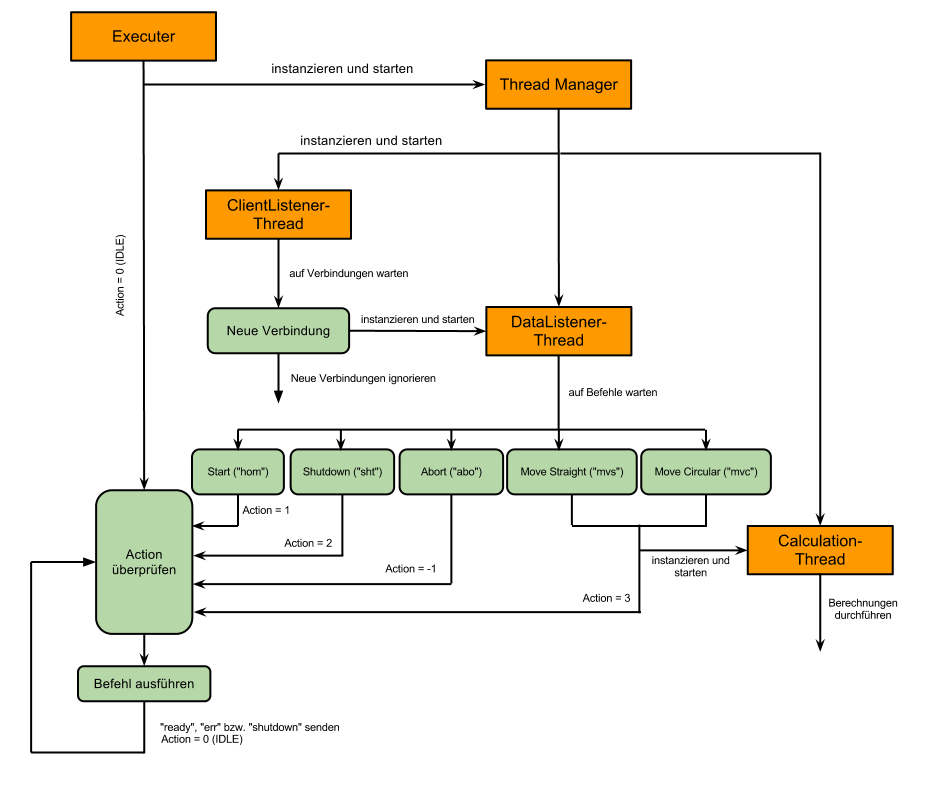
\includegraphics[width=14cm]{images/GHISteuerungssoftware}
\caption{Der Aufbau der Steuerungssoftware}
\end{figure}

\subsubsection{Die Executer Klasse}
Die Klasse \textit{Executer} ist die Basiskompente der Steuerungssoftware. Sie beinhaltet die Main Methode und wird bei Programmstart ausgeführt.
Auf Grund der beschränkten Multithreading Möglichkeiten des .Net Micro Framworks müssen alle zeitkritischen Operationen im Hauptthread durchgeführt werden. Der Haupthread ist jener Thread der zu Beginn die \textit{Main()} der Klasse \textit{Executer} Methode aufruft.

Die Aufgabe dieser Klasse ist unter Anderem die Verwaltung zahlreicher statischer Variablen die dafür sorgen dass zentrale Daten aus allen Threads verwendet werden können.
Des weiteren befindet sich in der \textit{Main()} Methode dieser Klasse die Programmlogik die zur Initialisierung, sowie zur Erzeugung einer Instanz der Kasse \textit{ThreadManager} und zur Ausführung der dort definierten Methode \textit{StartThreads()} benötigt wird.

Die Klasse \textit{Executer} wurde als statische Klasse implementiert da sie die beim Programmstart auszuführende Klasse ist. Üblicherweise ist diese Klasse bereits beim Anlegen eines neuen Projektes vorhanden.

In der Klasse selbst befinden sich zahlreiche Deklarationen von öffentlichen statischen Objekten die von den verschiedenen Threads gemeinsam genutzt werden.

Die folgende Aufzählung beschreibt die einzelnen Methoden der \textit{Executer} Klasse genauer.

\begin{itemize}
\item \textbf{Main() - Methode}\\
Die Main Methode der \textit{Executer} Klasse weist einigen der beschriebenen statischen Objekte Werte zu und aktiviert beispielsweise die Netzwerkschnittstelle.

Bei der Initialisierung werden auch zwei statische Objekte der Klasse \textit{Engine} instanziert. Ein Objekt dieser Klasse stellt in Form von Objekten der GHI internen Klasse \textit{OutputPin} den Zugriff auf die benötigten Pins des jeweiligen Motors bereit. Die Auswahl des durch das \textit{Engine} Objekte abgebildeten Motors geschieht beim Anlegen über den Konstruktor (\textit{Integer} Wert: 1 für primaren Motor, 2 für sekundären Motor). Der Konstruktor initialisiert hierbei die jeweils benötigten Pins als \textit{OutputPin} Objekte und macht sie öffentlich zugreifbar.

Wurde in der \textit{Main()} Methode eine Instanz der \textit{NetworkManager} Klasse erzeugt und die dazugehörige Methode \textit{StartThreads()} aufgerufen, Gerät der Hauptthread in der \textit{Main()} Methode der \textit{Executer} Klasse in eine Dauerschleife welche durchwegs den aktuellen Wert der statischen Variable \textit{action} überwacht und bei Änderung mithilfe eines \textit{Switch}-Konstrukts die jeweilige gewählte Aufgabe erledigt.

\item \textbf{Move() - Methode}\\
Ebenfalls in der \textit{Executer} Klasse befindet sich die Methode \textit{Move()}. Sie befindet sich hier, da es sich hierbei um eine einen zeitkritischen Vorgang ausführende Methode handelt und diese damit im höher priorisierten Hauptthread des Programms laufen muss.

Die \textit{Move()} Methode ist für die Ausgabe des Taktes und damit der Geschwindigkeit, sowie Einstellung der Richtung über das setzen des entsprechenden Ausgangsports verantwortlich.

Um dieser Aufgabe gerecht zu werden läuft die Methode mithilfe von Schleifen durch einzelne Arrays welche die aufbereiteten Daten der anzufahrenden Punkte in Form von Integer Werten enthalten. Die Arrays werden durch einen anderen Thread befüllt und enthalten die Anzahl der zu fahrenden Takte pro Interpolationsschrit, sowie \textit{boolean} Werten für die Richtung der Bewegungen.
Die beschriebenen Arrays befinden sich in Form von statischen Objekten in der \textit{Executer} Klasse.

Wie erwähnt stellen die einzelnen Werte in den statischen Arrays jeweils die Schrittzahlen dar die zum Erreichen eines Punktes (beispielsweise eines Interpolationspunktes zum Fahren einer Gerade) je Motor gefahren werden müssen. Beim durchlaufen dieser Arrays wird jeweils zuvor die benötigte Richtung - \textit{true} (im Uhreigersinn) oder \textit{false} (gegen den Uhrzeigersinn) - durch setzen des entsprechenden Richtungspins über das \textit{OutputPin} Objekt \textit{engineDir} des jeweiligen Engine Objektes.

Im nächsten und wichtigsten Schritt werden die einzelnen Takte an die Schrittmotorsteuerung übermittelt. Ein Takt wird immer dann durch die Schrittmotorsteuerung gefahren, wenn an dem entsprechenden Port eine positive Spannungsrampe erkannt wird. Daher ist es nötig für jeden Schritt jeweils zuerst die \textit(Write()) Methode des \textit{OutputPort} Objekts eines Motors mit \textit{false} und dann mit \textit{true} aufzurufen.

Wie bereits erwähnt befinden sich die Informationen zu den anzufahrenden Punkten in einzelnen statischen Integer Arrays. Für jeden Motor existiert hierbei ein Array mit einer Liste der jeweils zu fahrenden Takte. In einer Schleife wird nun dieses Array durchlaufen und für jeden darin enthaltenen Takt ein Takt an die Motorsteuerung übergeben.

Um eine geradlinige Bewegung zu erzeugen müssen jeweils die zwei Werte in den Array die den selben Index besitzen gleichzeitig abgearbeitet werden und es muss auf die Synchronisation der beiden Motoren geachtet werden. Dies geschieht mit Hilfe einer Variable \textit{rel} des Typs \textit{double} die das Verhältnis der Schritte eines Wertpärchens (Werte mit gleichem Index) darstellt. In der Schleife welche die Einzelnen Schritte an den Pins ausgiebt werden die Relation der einzuhaltenden Pausen zwischen den Schritten eines jeweiligen Motors mithilfe dieser \textit{rel} Variable berechnet.
\begin{lstlisting}[language = csharp, captionpos=b, caption={Beispiel für die Motorsynchronisation}]
			rel = (double)secondarySteps[i] / (double)primarySteps[i];

			small_count += rel;

                            if (rel > 0.5 && small_count > 1)
                            {
                                small_count = small_count % 1;
                                secondaryEngine.engineFreq.Write(true);
                                secondaryEngine.engineFreq.Write(false);
                            }
                            else
                            {
                                if (rel <= 0.5 && small_count > 0.5)
                                {
                                    small_count = 0;
                                    secondaryEngine.engineFreq.Write(true);
                                    secondaryEngine.engineFreq.Write(false);
                                }
                            }

                            primaryEngine.engineFreq.Write(true);
                            primaryEngine.engineFreq.Write(false);
                            j++;
\end{lstlisting}

Wurden alle in den Arrays befindlichen Interpolatinspunkte abgefahren, so wird über das \textit{clientsocket} Objekt die Zeichenkette "'ready"' an den Computer zurückgegeben um das Senden weiterer Befehle freizugeben.

\end{itemize}

\subsubsection{Die Engine Klasse}

Die Hauptaufgabe der Engine Klasse ist die Verwaltung einzelner Motoren. Dafür initialisiert sie im Konstruktor die benötigten \textit{OutputPin} Objekte mit den richtigen Pins für den über einen \textit{Integer} Parameter angegebenen Motor. In der derzeitigen Ausbauphase verfügt Edubot lediglich über zwei Motoren, aus diesem Grund können als Parameter für den Konstruktor entweder die Zahl 1 - für den Motor der primären Achse und die Zahl 2 - für den Motor der Sekundären Achse mitgegeben werden.

Die einzelnen \textit{OutputPin} Objekte werden mit Standardwerten initialisiert. Es werden folgende Pins initialisiert und für die aufgelisteten Variablen werden die daneben aufgelisteten Standardwerte gesetzt:

\begin{table}[h]
\begin{tabular}{|p{3cm}|p{3.5cm}|p{3.5cm}|p{3.5cm}|}
\hline \rowcolor{lightgray}
\textbf{Variablenname} & \textbf{Funktion} & \textbf{Standardwert} &\textbf{Pin}\\
\hline
engineEnabled & Ein-/Ausschalten des Motors & false, Motor ist eingeschaltet & primary: EMX.Pin.IO0 secondary: EMX.Pin.IO4\\
\hline
engineFreq & Taksignal, bei positiver Spannungsrampe wird ein Schritt gefahren & false & primary: EMX.Pin.IO2 secondary: EMX.Pin.IO6\\
\hline
engineDir & Richtung in die Schritte gefahren werden & false, gegen den Uhrzeigersinn & primary: EMX.Pin.IO1 secondary: EMX.Pin.IO5\\
\hline
enginePowerDown & Ein-/Ausschalten der Automatischen Stromabsenkung bei Stillstand & false, Spannungsabsenkung ist aktivert & primary: EMX.Pin.IO3 secondary: EMX.Pin.IO7\\
\hline
\end{tabular}
\caption{Motorpins und Standardwerte}
\end{table}

Um nun auf eine der genannten Funktionen eines Motors Zugriff zu bekommen benötigt man lediglich eine Instanz der Engine Klasse die dem gewünschten Motor entspricht. Setzt man nun beispielsweise mit dem folgenden Aufruf auf den \textit{engineEnabled} Pin auf \textit{true}, so gibt der Motor am entsprechenden Pin eine Spannung von 5V aus und der Motor wird ausgeschaltet. (Die Schrittmotorsteuerung schaltet den Motor aus wenn Spannung anliegt und nicht umgekehrt)
\begin{lstlisting}[language = CSharp, captionpos=b, caption={Das Setzen eines OutputPins}]
engineEnabled.Write(true);
\end{lstlisting}
 
\subsubsection{Die ThreadManager Klasse}
Da für das gleichzeitige Empfangen, Extrahieren und Ausgeben von Interpolationsschritten mehrere Threads benötigt werden, gibt es in der Software des Mikrocontrollers eine eigene Klasse \textit{ThreadManager}. Sie beinhaltet sowohl die Methoden zum extrahieren der Takte aus der Empfangenen Zeichenkette, als auch alle Methoden die für die Kommunikation mit dem PC benötigt werden.

Die \textit{ThreadManager} Klasse beinhaltet einzelne Methoden die während des Betriebs parallel ausgeführt werden müssen. Um dies zu bewerkstelligen startet die Methode jeweils zur Ausführung einer Methode einen neuen Thread. Zusätzlich zu den Methoden enthält die Klasse das für das horchen auf Verbindungen benötigte \textit{Socket} Objekt \textit{server}.

Die Netzwerkkommunikation zwischen Mikrocontroller ist auf Sockets aufgebaut und verwendet das TCP Protokoll, wobei der Mikrocontroller selbst als Server agiert und sich angeschlossene PCs als Clients verbinden könen

Die folgende Auflistung gibt einen groben Überblick, welche Methoden in der \textit{ThreadManager} Klasse enthalten sind und wie sie funktionieren.

\begin{itemize}
\item \textbf{ListenForClients() - Methode}\\
Wird die \textit{StartThreads()} Methode eines \textit{ThreadManager} Objekts aufgerufen, so wird für die Methode \textit{ListenForClients()} ein neuer Thread gestartet. Der frisch erzeugte Thread beschäftigt sich fortan in einer Dauerschleife mit dem Warten auf neue eingehende Verbindungen. Ist bereits eine aktive Verbindung vorhanden, so nimmt die Methode keine neuen Verbindungen an.

Versucht sich ein Client mit dem Mikrocontroller zu verbinden während der erklärte Thread auf Verbindungen horcht, so wird durch die \textit{Accept} Methode des \textit{server} Objekts welches im Konstruktor definiert wurde ein neuer Socket erzeugt der von nun an die aktive Verbindung repräsentiert und als statisches Objekt mit dem Namen \textit{clientsocket} in der \textit{Executor} Klasse gespeichert wird.

\item \textbf{ListenForData() - Methode}\\
Wurde die neue Verbindung erfolgreich aufgebaut erzeugt die Methode \textit{ListenForClients()} einen neuen Thread für das empfangen von Daten über die neue Verbindung. Die Methode die durch den neuen Thread ausgeführt wird heißt\textit{ListenForData()} und wartet solange die Verbindung von \textit{clientsocket} besteht auf übertragene Daten. 
Die Information ob eine Verbindung besteht wird durch die statische \textit{boolean} Variable \textit{acceptNewClient} der Klasse \textit{Executer} global zur Verfügung gestellt und hält beispielsweise auch die \textit{ListenForClients()} Methode davon ab neue Verbindungen zu akzeptieren.

Die Methode \textit{ListenForData(}) fragt mit einer Schleife, solange die Verbindung besteht, beim  \textit{clientsocket} Objekt nach ob neue Daten für den Empfang bereitstehen. Ist dies der Fall, so werden diese als Byte Array geladen und danach in eine Zeichenfolge konvertiert.

Ebenfalls in der \textit{ListenForData()} Methode wird auf Basis des Präfix in den ersten drei Zeichen der Nachricht entschieden welche Operation als nächstes ausgeführt wird (Homing, LinearMovement, CircularMovement etc.) und die \textit{action} Variable der Executer Klasse entsprechend gesetzt. Durch setzen \textit{action} Variable wird im Haupthread beispielsweise die Move() Methode aufgerufen.

Wurde vom Client eine Operation angefordert welche die Extraktion der zu Verfahrenden Schritte aus den empfangenen Daten voraussetzt (beispielsweise LinearMovement), so wird ein neuer Thread mit der Methode \textit{Calculate()} erzeugt, der nun beginnt die einzelnen Taktanzahlen aus der empfangene Zeichenkette zu extrahieren zurechnen.

\item \textbf{Calculate() - Methode}\\
Wie oben beschrieben wird diese Methode in einem eigenständigen Thread aufgerufen um Empfangene Daten aus der vom Client gesendeten Zeichenkette zu extrahieren und die statisch in der \textit{Executer} Klasse gespeicherten Arrays mit den Informationen zu den Taktzahlen von Teilstrecken sowie den dazugehörigen Richtungen mit zu befüllen. 
Hierzu wird mithilfe der \textit{Split()} Methode der \textit{String} Klasse die gesamte Zeichenkette in einzelne Interpolationsschritte geteilt, aus welchen wiederum ebenfalls mit der \textit{Split()} Methode die Takte die jeder Motor für diesen Interpolationsschrit fahren muss extrahiert werden.

Während dieser Umwandlung, ruft der Hauptthread in der \textit{Move()} Methode der \textit{Executer} Klasse bereits Daten aus den Arrays ab und gibt sie an die Schrittmotorsteuerungen aus. Mehr dazu im Unterkapitel "Die Klasse Executer" unter dem Punkt "Move() - Methode".

\end{itemize}
\subsubsection{Der Homing Algorithmus}
Da nach dem Herstellen einer Verbindung mit dem Mikrocontroller nicht bekannt ist in welcher Position sich das Edubot Modell befindet, muss zuerst das sogenannte "'Homing"' durchgeführt werden. Dazu wurden am Edubot Modell Kontakte angebracht, welche geschlossen werden wenn der Roboterarm an die Grenzen seines Arbeitsbereichs stößt. Wurde der besagte Kontakt hergestellt, so liegt an einem bestimmten Pin des Mikrocontrollers eine Spannung von 3,5V an. 

In der Software lässt sich das Homing nun vergleichsweise einfach lösen. Dazu fährt zunächst der sekundäre Motor, also der Motor des zweiten Arms, mittels einer Schleife so lange immer einen Schritt, bis die Achse an die Grenze ihres Arbeitsbereichs stößt. Mithilfe eines Objekts vom Type \textit{InputPin}, welches einen bestimmten Pin des Mikrocontrollers repräsentiert kann hierzu durch die Methode \textit{Read()} des Objekts jederzeit abgefragt werden ob Spannung an diesem Pin anliegt. Stößt die Achse an die Grenze ihres Arbeitsbereichs, so wird der oben beschrieben Kontakt geschlossen und die \textit{Read()} Methode des entsprechenden Pins gibt \textit{true} zurück, wodurch die Schleife beendet wird. Da sich die Achse immer nur im Uhrzeigersinn bewegt ist lediglich eine Kontaktstelle an der im Uhrzeigersinn befindlichen Grenze des Arbeitsbereichs nötig. 

\begin{figure}[H]
\centering
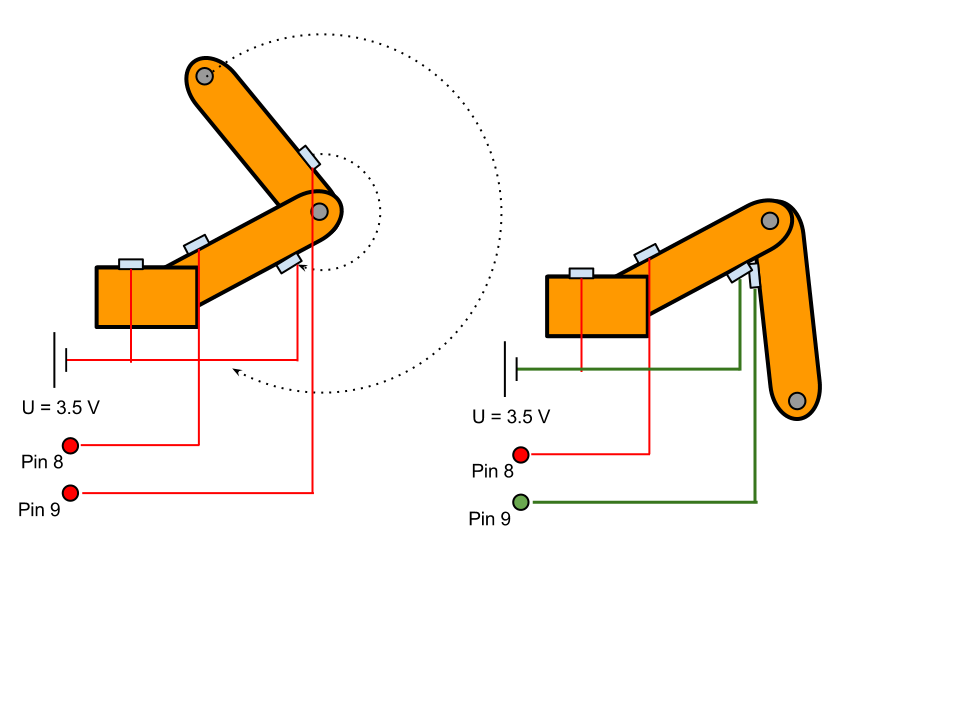
\includegraphics[width=11cm]{images/Homing}
\caption{Das Finden der Grenze der sekundären Achse}
\end{figure}

Befindet sich die sekundäre Achse im Ende ihres Arbeitsbereichs, so beginnt der primäre Motor den selben Prozess durchzuführen. In diesem Fall befindet sich die Kontaktstelle jedoch an der gegen den Uhrzeigersinn befindlichen Grenze des Arbeitsbereichs. Aus diesem Grund fährt dieser Motor in einer Schleife jeweils einen Takt gegen den Uhrzeigersinn und überprüft dann ob er bereits die Grenze erreicht hat.

\begin{figure}[H]
\centering
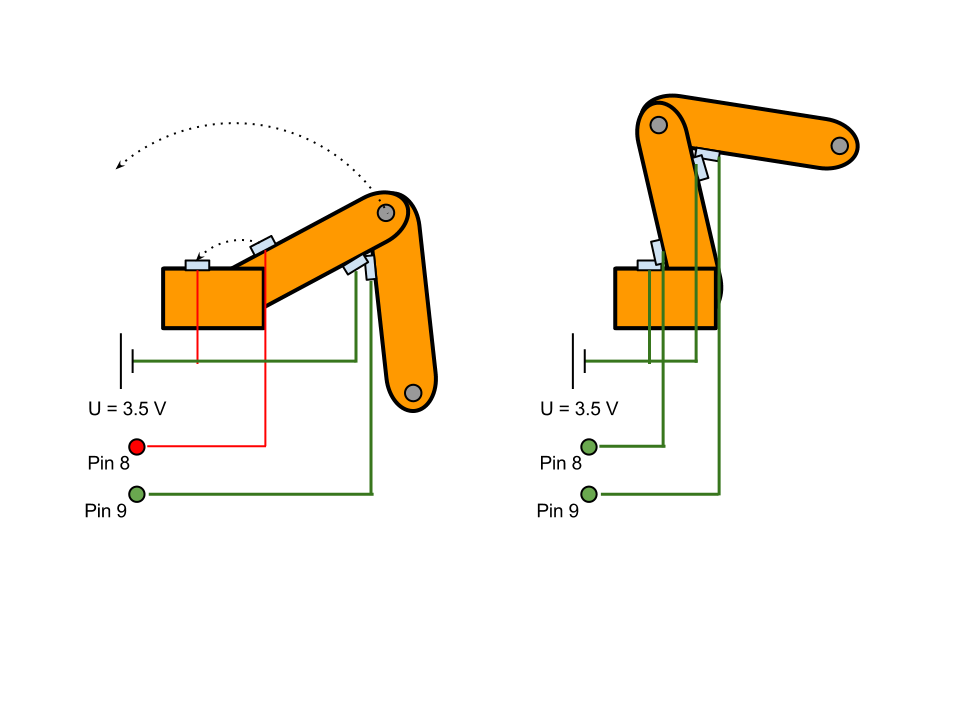
\includegraphics[width=11cm]{images/Homing2}
\caption{Das Finden der Grenze der primären Achse}
\end{figure}

Das eigentliche Fahren in die Ausgangsposition geschieht nun durch die Ausgabe einer für jeden Motor fix festgelegten Taktanzahl. Diese wurde bei der Entwicklung durch Versuche festgestellt und bringt die beiden Achsen in eine gerade Stellung. Die beiden Achsen fahren hierfür gleichzeitig, sind aber nicht synchronisiert und werden daher zu unterschiedlichen Zeitpunkten fertig. 

Wurde das "'Homing"' erfolgreich durchgeführt, wird über die Socket Verbindung die Zeichenkette "'ready"' an den Computer zurückgegeben um zu Signalisieren dass der Roboter für den Empfang weiterer Befehle bereit ist.
